大语言模型（LLM）正日益被部署来解决需要长交互序列的复杂工具使用任务，例如软件工程~\citep{jimenez2024swebench,jain2024livecodebench}和多步推理~\citep{wang2022scienceworld, yang2024sweagent,team2025tongyi,phan2025humanitysexam}。这类 LLM 的一个决定性特征是其长时程性：每个 episode 通常需要几十次顺序模型调用。随着轨迹变长，累积推理成本---又受到上下文窗口扩大~\cite{dao2023flashattention}和 token 消耗超线性增长~\citep{gao2025lessempiricalstudyturncontrol}的加剧---成为实际部署与可复现研究的主要障碍。

\begin{figure}[!tbp]
\centering
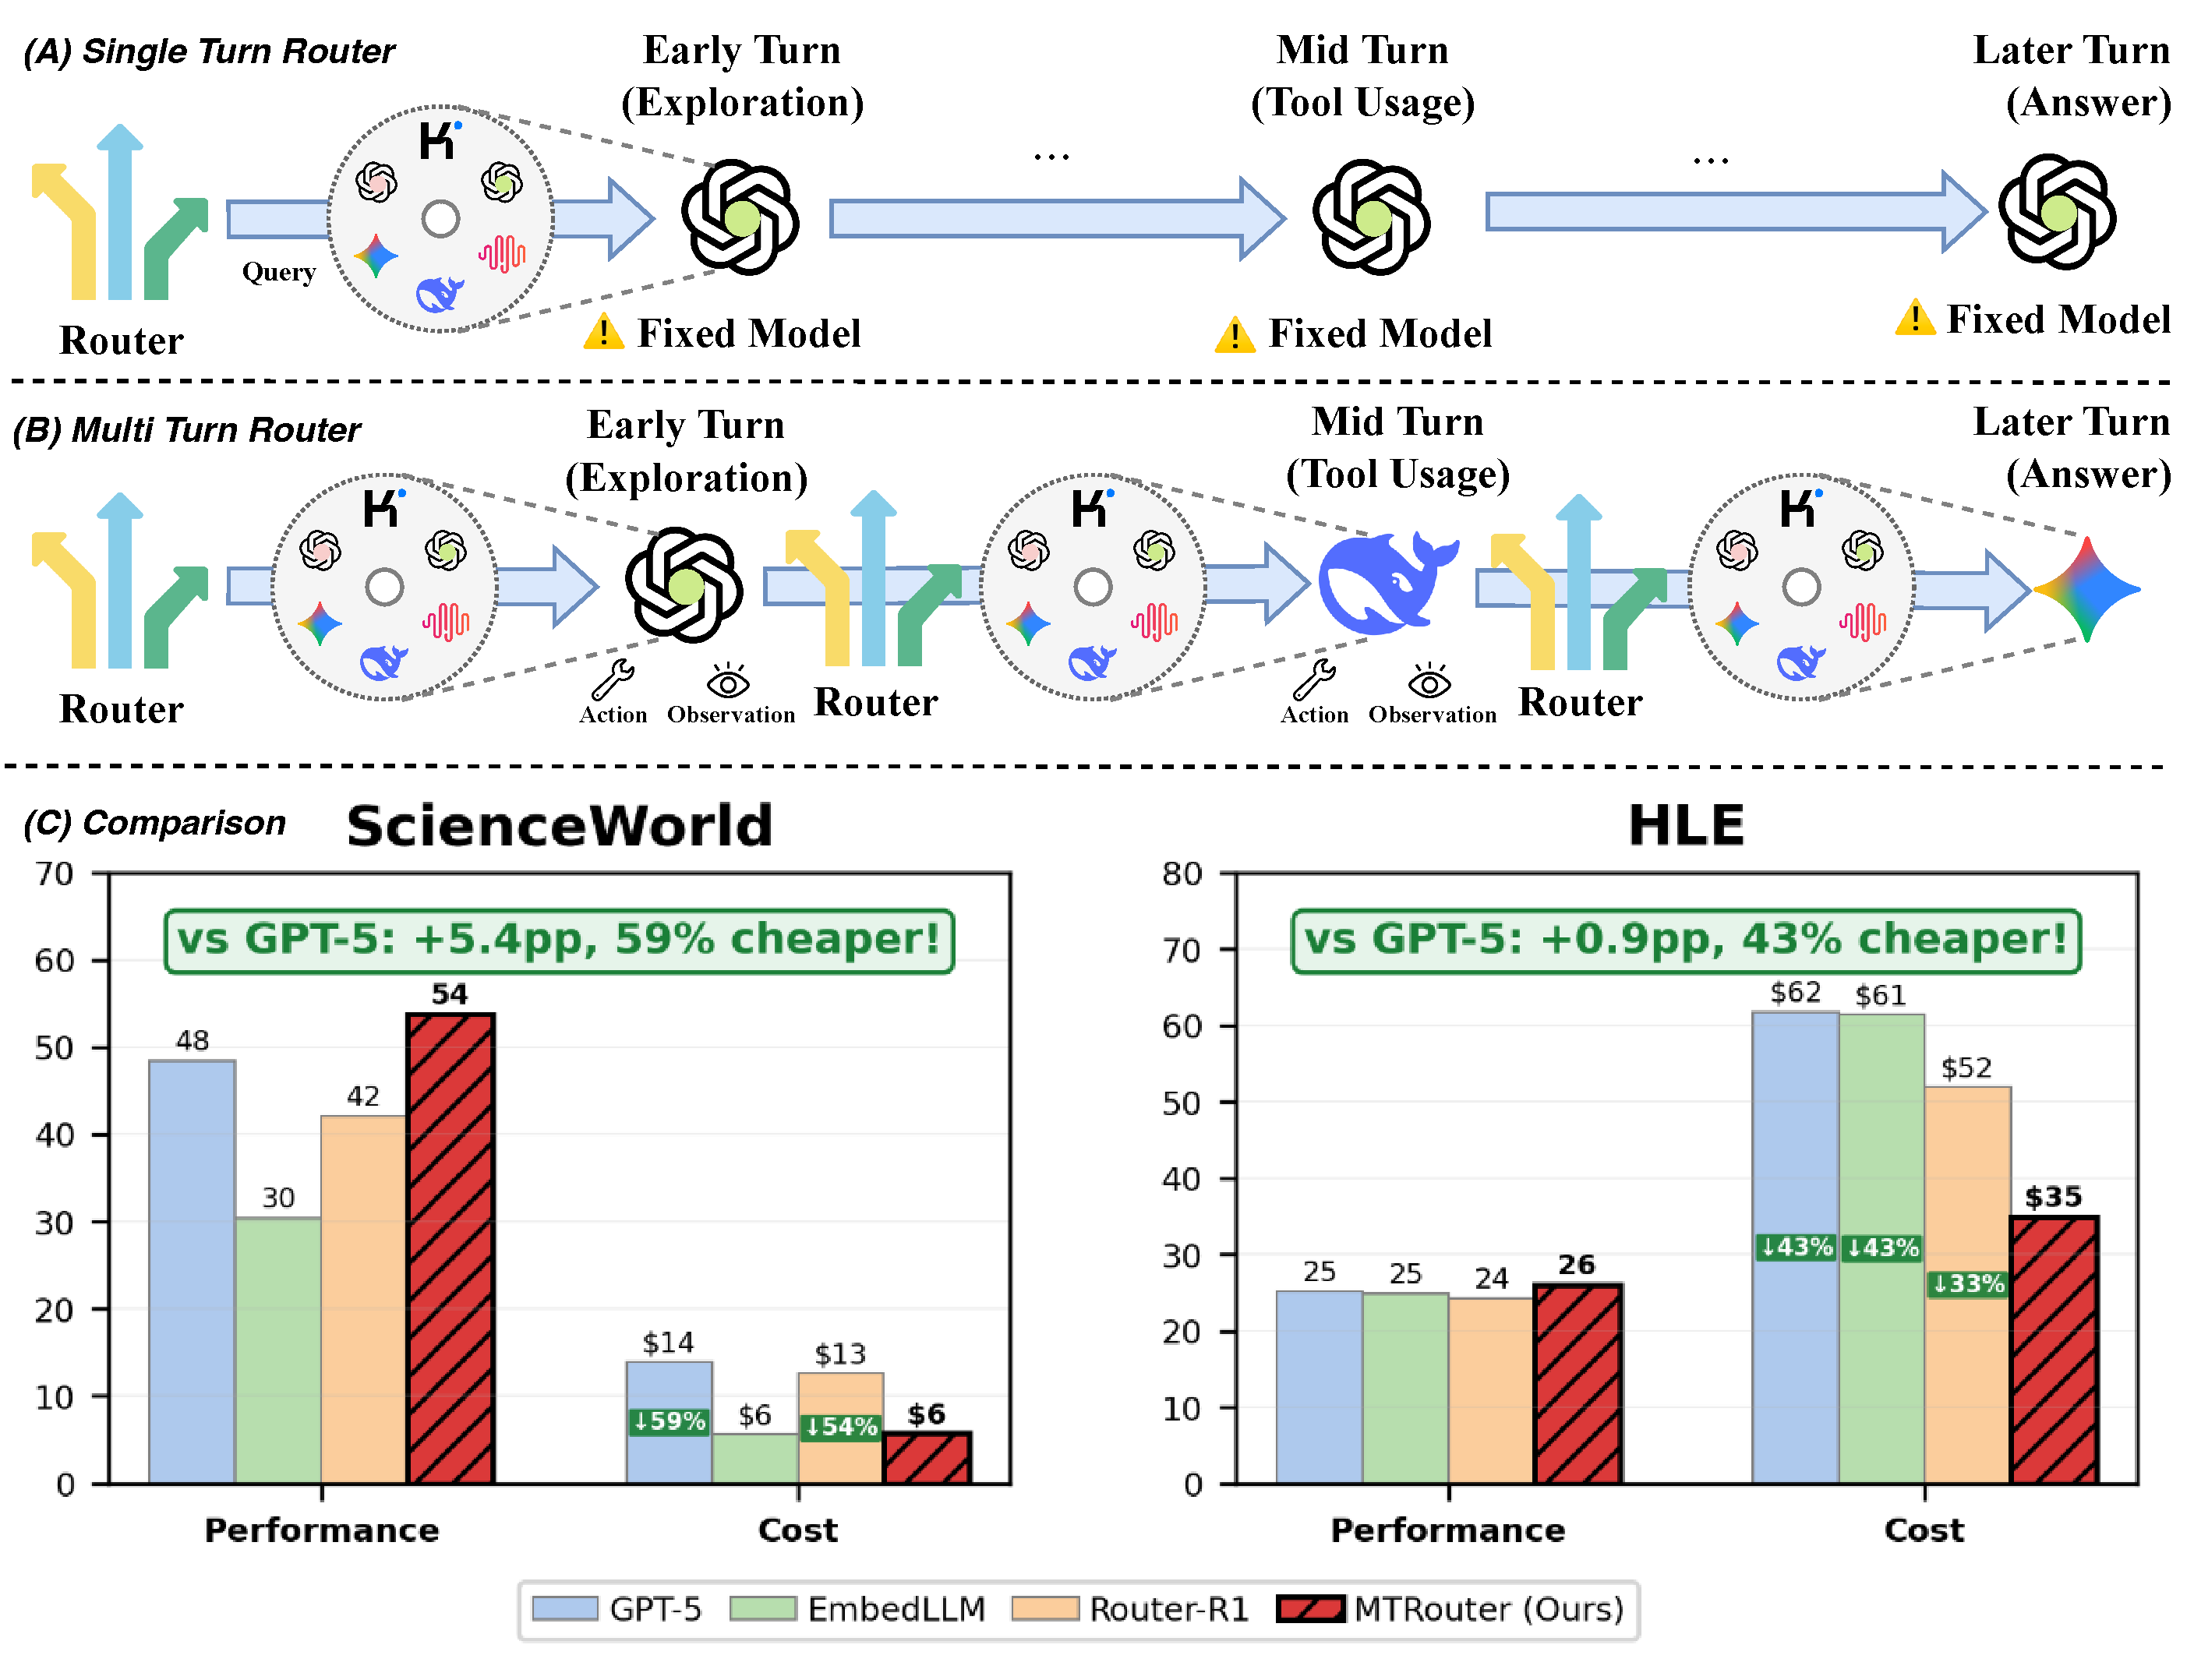
\includegraphics[width=\linewidth]{figures/toy-example.pdf}
\caption{\textbf{上：}单轮（episode 级）路由器选择一个模型，并在整个 episode 中保持不变。\textbf{中：}多轮路由器可随交互状态变化，在不同轮次调整模型选择。\textbf{下：}\method 在 ScienceWorld~\citep{wang2022scienceworld} 与 Humanity's Last Exam（HLE）~\citep{phan2025humanitysexam}上，比有代表性的基线取得更优的性能--成本权衡。}
\label{fig:toy_example}
\vspace{-1.0em}
\end{figure}

当前模型生态中存在显著的经济差距，这进一步加剧了这一压力：前沿模型提供最先进的推理能力（如 \texttt{claude-opus-4.5}\footnote{\url{https://www.anthropic.com/claude/opus}}、\texttt{gpt-5}\footnote{\url{https://openai.com/index/gpt-5-system-card}}），但成本通常比轻量模型高两个数量级（如 \texttt{DeepSeek-v3.2}~\citep{liu2025deepseek}、\texttt{Kimi-K2}~\citep{team2025kimi}）。为降低成本，已有工作探索了单轮（episode 级）路由：根据初始提示词在 episode 开始时选择一个模型（图~\ref{fig:toy_example}，上）。但这种静态方法对于长时程任务天然次优。一条 episode 通常包含异质步骤，从高风险的战略规划到例行工具调用和数据格式化。每一轮都使用前沿模型会造成浪费，而只依赖廉价模型则可能在关键节点引发灾难性失败。

这一观察促成了多轮（轮级）路由：智能体在交互的每一步自适应地切换模型（图~\ref{fig:toy_example}，中）。尽管有前景，多轮路由面临显著的预测挑战：路由器必须评估当前轮的一个特定模型选择，是否会在数十步之后危及最终结果。简单启发式规则或局部错误检测通常无法捕获模型表现对整条轨迹的长期影响。

我们提出 \textbf{\method}，它从已记录轨迹中学习一个\emph{结果估计器}。该估计器将历史--模型对映射为最终 episode 结果（终止得分/准确率）的估计，并通过考虑错误的调整从离线数据中获得稳定的训练信号。推理时，路由器在每一轮选择预测结果最高的候选模型，并在固定成本和轮数限制下评估 episode。

在实证上，\method 在性能和成本两方面均带来一致收益。在 ScienceWorld（测试集）上，它将平均得分从 48.4（GPT-5）提升至 53.8，同时将总成本降低 58.7\%；在 HLE（测试集）上，它以降低 43.4\% 总成本实现有竞争力的准确率。它还可在语义分布偏移（OOD）下泛化，以显著成本节省保持更好的结果（表~\ref{tab:combined_results}）。除汇总指标外，我们的分析还表明，多轮路由并不等于“更多切换”：\method 比 Router-R1~\cite{zhang2025router}以更少模型切换获得成功，对瞬时错误更具容忍性，并呈现结构化模型使用与跨工具/动作的涌现专长（图~\ref{fig:cost_switches}--\ref{fig:action_by_model}）。

我们的主要贡献如下：
\begin{itemize}[nolistsep, noitemsep, leftmargin=*]
\item 我们提出 \textbf{\method}：它从离线轨迹中学习历史--模型对上的结果估计器，并在多轮智能体 episode 中执行轮级路由。
\item 我们在 ScienceWorld 和 HLE（测试与 OOD）上以固定候选池开展评估，结果表明，相较包括 Router-R1 与有代表性的商用路由器在内的强基线，\method 在性能和总成本上均有一致改善。
\item 我们提供分析，将这些收益关联到具体路由行为，包括更少不必要的切换、更好的错误恢复，以及跨工具/动作的涌现专长。
\end{itemize}
